\subsection{Background and motivation}
    % context, setting - B2C business gathers a lot of data
    Many software businesses collect enormous amount of data generated by end-users \cite{chinesemobilebankingusers, bigdatamanagementrevolution, inmon2007tapping}. End-user data incorporates essential information about how users interact with the system of discussion as well as tells a lot about the users themselves \cite{jang2015noreciprocity, hu2014we, jang2016teensengagemorewithfewerphotos, han2016teensarefrommars, socialdiversityongithub}. For instance, such data can explain the preferences of users, what kind of content they like, how they interact with the system and eachother or how frequently they use the software that has generated the data \cite{youyou2015computer, ottoni2013ladies}.
    
    % what is the challenge?
    Depending on the portfolio of the business, analysis of end-user data can reveal various interesting findings. For instance, in banking industry Big Data tools are often used to analyze demographic characteristics to maintain and establish new client relationships \cite{chinesemobilebankingusers, bigdatamanagementrevolution}. Extracting the information from the data is challenging: most businesses are to collect more data than what is humanly possible to process and to analyze \cite{inmon2007tapping, wegener2010integrating}. As a result, significant part of the knowledge might remain hidden and hence business-critical information remains unseen \cite{inmon2007tapping, wegener2010integrating, introtodatamining, chinesemobilebankingusers}. The computational methods of today's world enable us not only to achieve previously impossible tasks, but also to create tools that may outperform humans \cite{youyou2015computer}. Accordingly, there is a growing need for all businesses to introduce data analysis processes in their daily activities with the aim of understanding users and data generated by them better.
    
    % how do mobile devices have an impact on the amount of data? 
    With the continuous growth of mobile devices in numbers, the amount of generated data has increased significantly. Due to the wide availability and commonness of smartphones and tablets, anybody can easily generate rich location, media or textual data \cite{jang2016teensengagemorewithfewerphotos}. Complementary to the popularity of mobile devices, social media sites have grown a lot in the past years \cite{ottoni2013ladies, hu2014we, bakhshi2014faces, waheed2017investigation}, allowing users rich ways of interaction. Due to the combination of these two trends, users leave digital footprints in form of location, media, numerical or textual data in numerous places around the Internet \cite{youyou2015computer}. People often express their opinion by sharing, liking or commenting on data over social networks. Based on this information, algorithms can predict their personality traits more reliably than other humans would do \cite{youyou2015computer}. These facts further increases the call for research in the field of mobile and user data analysis, because it can help researchers to understand the society, human behavior, preferences and public opinions better.

	% what is the potential in analyzing user data? why is it important not only to collect but also analyze data?
    Data analysis tools and methods already exist to help businesses to process user data. However, these applications often not utilized, because companies rather focus on developing their service package than understanding the previously gathered data \cite{inmon2007tapping, bigdatamanagementrevolution}. As a result, essential knowledge concerning previously collected data is neglected, which would be key for the future development of the business. Careful data analysis may reveal interesting relationships and point out facts, what human eyes would never notice otherwise \cite{bigdatamanagementrevolution}. Consequently, Knowledge Discovery in Databases is important and is essential part of Business Intelligence applications as well \cite{zarsky2002mine, bigdatamanagementrevolution}. 
    
    % what is the goal? what is this thesis about?
    The goal of this research is to study understand the potential use of user data in business and research environments in the present time with the application of Data Mining methods. The research aims to study how content on the Internet is observed by the users, who access the content. Secondly, it is studied what kind of feedback is received from the engaged audience in terms of like activities and comments to the provided content. Thirdly, the tendencies among the demographic characteristics between users are studied in relation to the content which gets them engaged online. More specifically, the Choicely voting/audience engagement platform is taken as a case study. Association analysis, statistical methods and computer vision are utilized to understand the online content and to reveal yet unseen details about the tendencies of user preferences in terms of votes spent on contest participants in the platform.
    
    % why is this research conducted, what is the motivation from researcher's pov? 
    One reason behind conducting this research are the stimulating challenges about studying user data and the wide possibilities of the information that may lie around in databases. Previous research have proven the relevance of statistical analysis on Big Data, such as like activities \cite{jang2015noreciprocity, jang2016teensengagemorewithfewerphotos, ottoni2013ladies, guy2016whatsyourorganizationlike, jang2015no, youyou2015computer}, user comments \cite{jang2016teensengagemorewithfewerphotos}, tags \cite{jang2016teensengagemorewithfewerphotos}, image content \cite{hu2014we, bakhshi2014faces} and movie ratings \cite{saraee2004data, kabinsingha2012movie} by revealing interesting findings about user behavior. Moreover, as service providers often get access to user demographics-related data through social network sites in the present time, new possibilities become available to seek correlation between user segments. Studies conducted in this field are also interesting from the point of view of human behavior research, which is another motivation towards conducting studies in this area. 

    \pagebreak

    % what is the motivation behind the focus from Choicely's point of view? 
    From the perspective of the case company and its customers such research is interesting, because it helps the company's management and customers to 

    \begin{itemize}
        \item understand the composition of their engaged user base better,
        \item have more advanced quantifiable means on the collected data,
        \item gain an understanding on the users' behavior, 
        \item increase business value.
    \end{itemize} 

\subsection{Research questions, scope and objectives}
In this chapter, the research questions, scope and objectives are presented and explained. The most important research questions are as follows:

    \begin{enumerate}[label=RQ\arabic*:]
        \item \textbf{How is user data understood and utilized in previous research?} The aim of this research question is to discover the conceptual understanding and potential development areas of user data based on related studies. The scope of the concept is defined and it is discussed, how other researchers have utilized the concept in the past.
        
        \item \textbf{What kind of content is more engaging for users and draws the most attention in the Choicely platform?} The aim of this research question is to understand which type of voting contests tend to engage more audience. Secondly, the question targets to analyze the attributes of those contestants, who received high number of votes. In other words, the aim is to find common features of contestants, who are highly rated by public opinion.

        \item \textbf{What are the behavioral characteristics of users by location and gender?} This research question targets to answer the question how users tend to use the platform. This covers the analysis of what kind of content users seek, how the votes are spent and what similarities can be observed in the data. To gain more specific understanding, the users will be grouped by their gender and location data.

        %\item \textbf{How is it possible to identify anomalies, such as peaks in or fraud usage from the data?}

        %\item \textbf{How is it possible to recommend relevant content for users based on prior user data?} The question targets to investigate and develop methods which can help users to find new content in the platform relevant to their interests.
    \end{enumerate}

    % what is the wide scope of the thesis? What will we begin with as a theoretical background?
    Initially, the study presents an overview on the field of user data analysis in different areas of research as the theoretical part of the study. Particularly, the study addresses the possibilities and challenges of analyses performed on user data in software applications, where users express their opinion via the usage of the system. For example, one can think of like activities on social media, reviewing movies online or voting on their favorite moment of a football match.

    % in what context is this theoretical background relevant? Answer "Why?" % how does that relate to Choicely, particularly? 
    Building on top of the theoretical framework, the study is oriented towards applying techniques for data mining purposes at Choicely. Being a large field of science, the scope is focused only on the most important portion of Data Mining techniques and methods, that are utilized to answer the research questions of this study. Specific topics from the field of Data Science are chosen to obtain the answers to the research questions. 
    
    % how does it relate to the case company?
    At the beginning of this research project, the company does not utilize any advanced data analysis tools. This thesis work is motivated in the direction to establish the basis of a data mining framework at the company and hence increase the business value of the firm.  

    % what is the objective? 
    One of the objectives of this thesis work is to develop advanced data analysis tools in order to assist the case company and its customers to gain a better understanding on the data at hand. In order to do that, the available data is presented and analyzed, the most interesting questions are stated and the information with more influential business value is identified. Afterwards, potential data analysis methods are discussed which are capable to retrieve such information from the given data set.  

    % what is the focus?
    More specifically, the research is oriented towards applying Data Mining techniques to gain a better understanding on the users and their level of engagement. Initially, the study is oriented towards discovering what kind of computational methods were applied in related studies to analyze properties of the user data. In the second part of the study, a chosen set of Data Mining techniques are utilized to discover the attributes of the content, which tends to engage a wider range of users. Finally, the behavior of different demographic user groups is studied in the Choicely platform in terms of their activities and what kind of differences can be identified among the different user groups.
    % Computer vision is utilized to classify the content of the images that are uploaded to the platform, while the transactional user data is investigated using association analysis techniques. % TODO finish when clarified

\subsection{Introduction to the Choicely voting platform}
    % what does the company do? 
    Choicely\footnote{\url{http://choicely.com/}} is a voting platform developed by the Finnish Lovented Ltd since 2014. The software provides the possibility for users to engage in interesting contests by voting on their favorite contender. The platform has already hosted numerous contests in various fields, such as beauty pageants, public polls, design contests, talent shows, sport events among many others. The customer base of the firm consist of mainly Finnish broadcasters, publishers and advertisers. However, the recent years have brought numerous users and customers from all around the world.

    % how can one reach a contest in the platform?
    Contests can be accessed through multiple interfaces (Figure \ref{choicely_platforms}). Naturally, the company's webpage provides a convenient way to create, browse and participate in contests. Choicely also has free mobile applications available on Android and iOS devices, that can be installed through the Google Play\footnote{\url{https://play.google.com/store/apps/details?id=com.choicely.android}} and the iOS App Store\footnote{\url{https://itunes.apple.com/fi/app/choicely/id1158798364}} on the devices. Finally, the company offers a web widget, which can be embedded as a framework in any webpage easily. The last option is often used by many of Choicely's customers, because it provides a convenient way to embed rich content in their own web pages, which users are already familiar with. Users may vote and participate in their own contests if they like. Users may participate in arbitrary number of contests from three platforms: the two most popular mobile platforms (iOS and Android) and the web interface. 

    \begin{figure}[h] 
        \begin{center}
            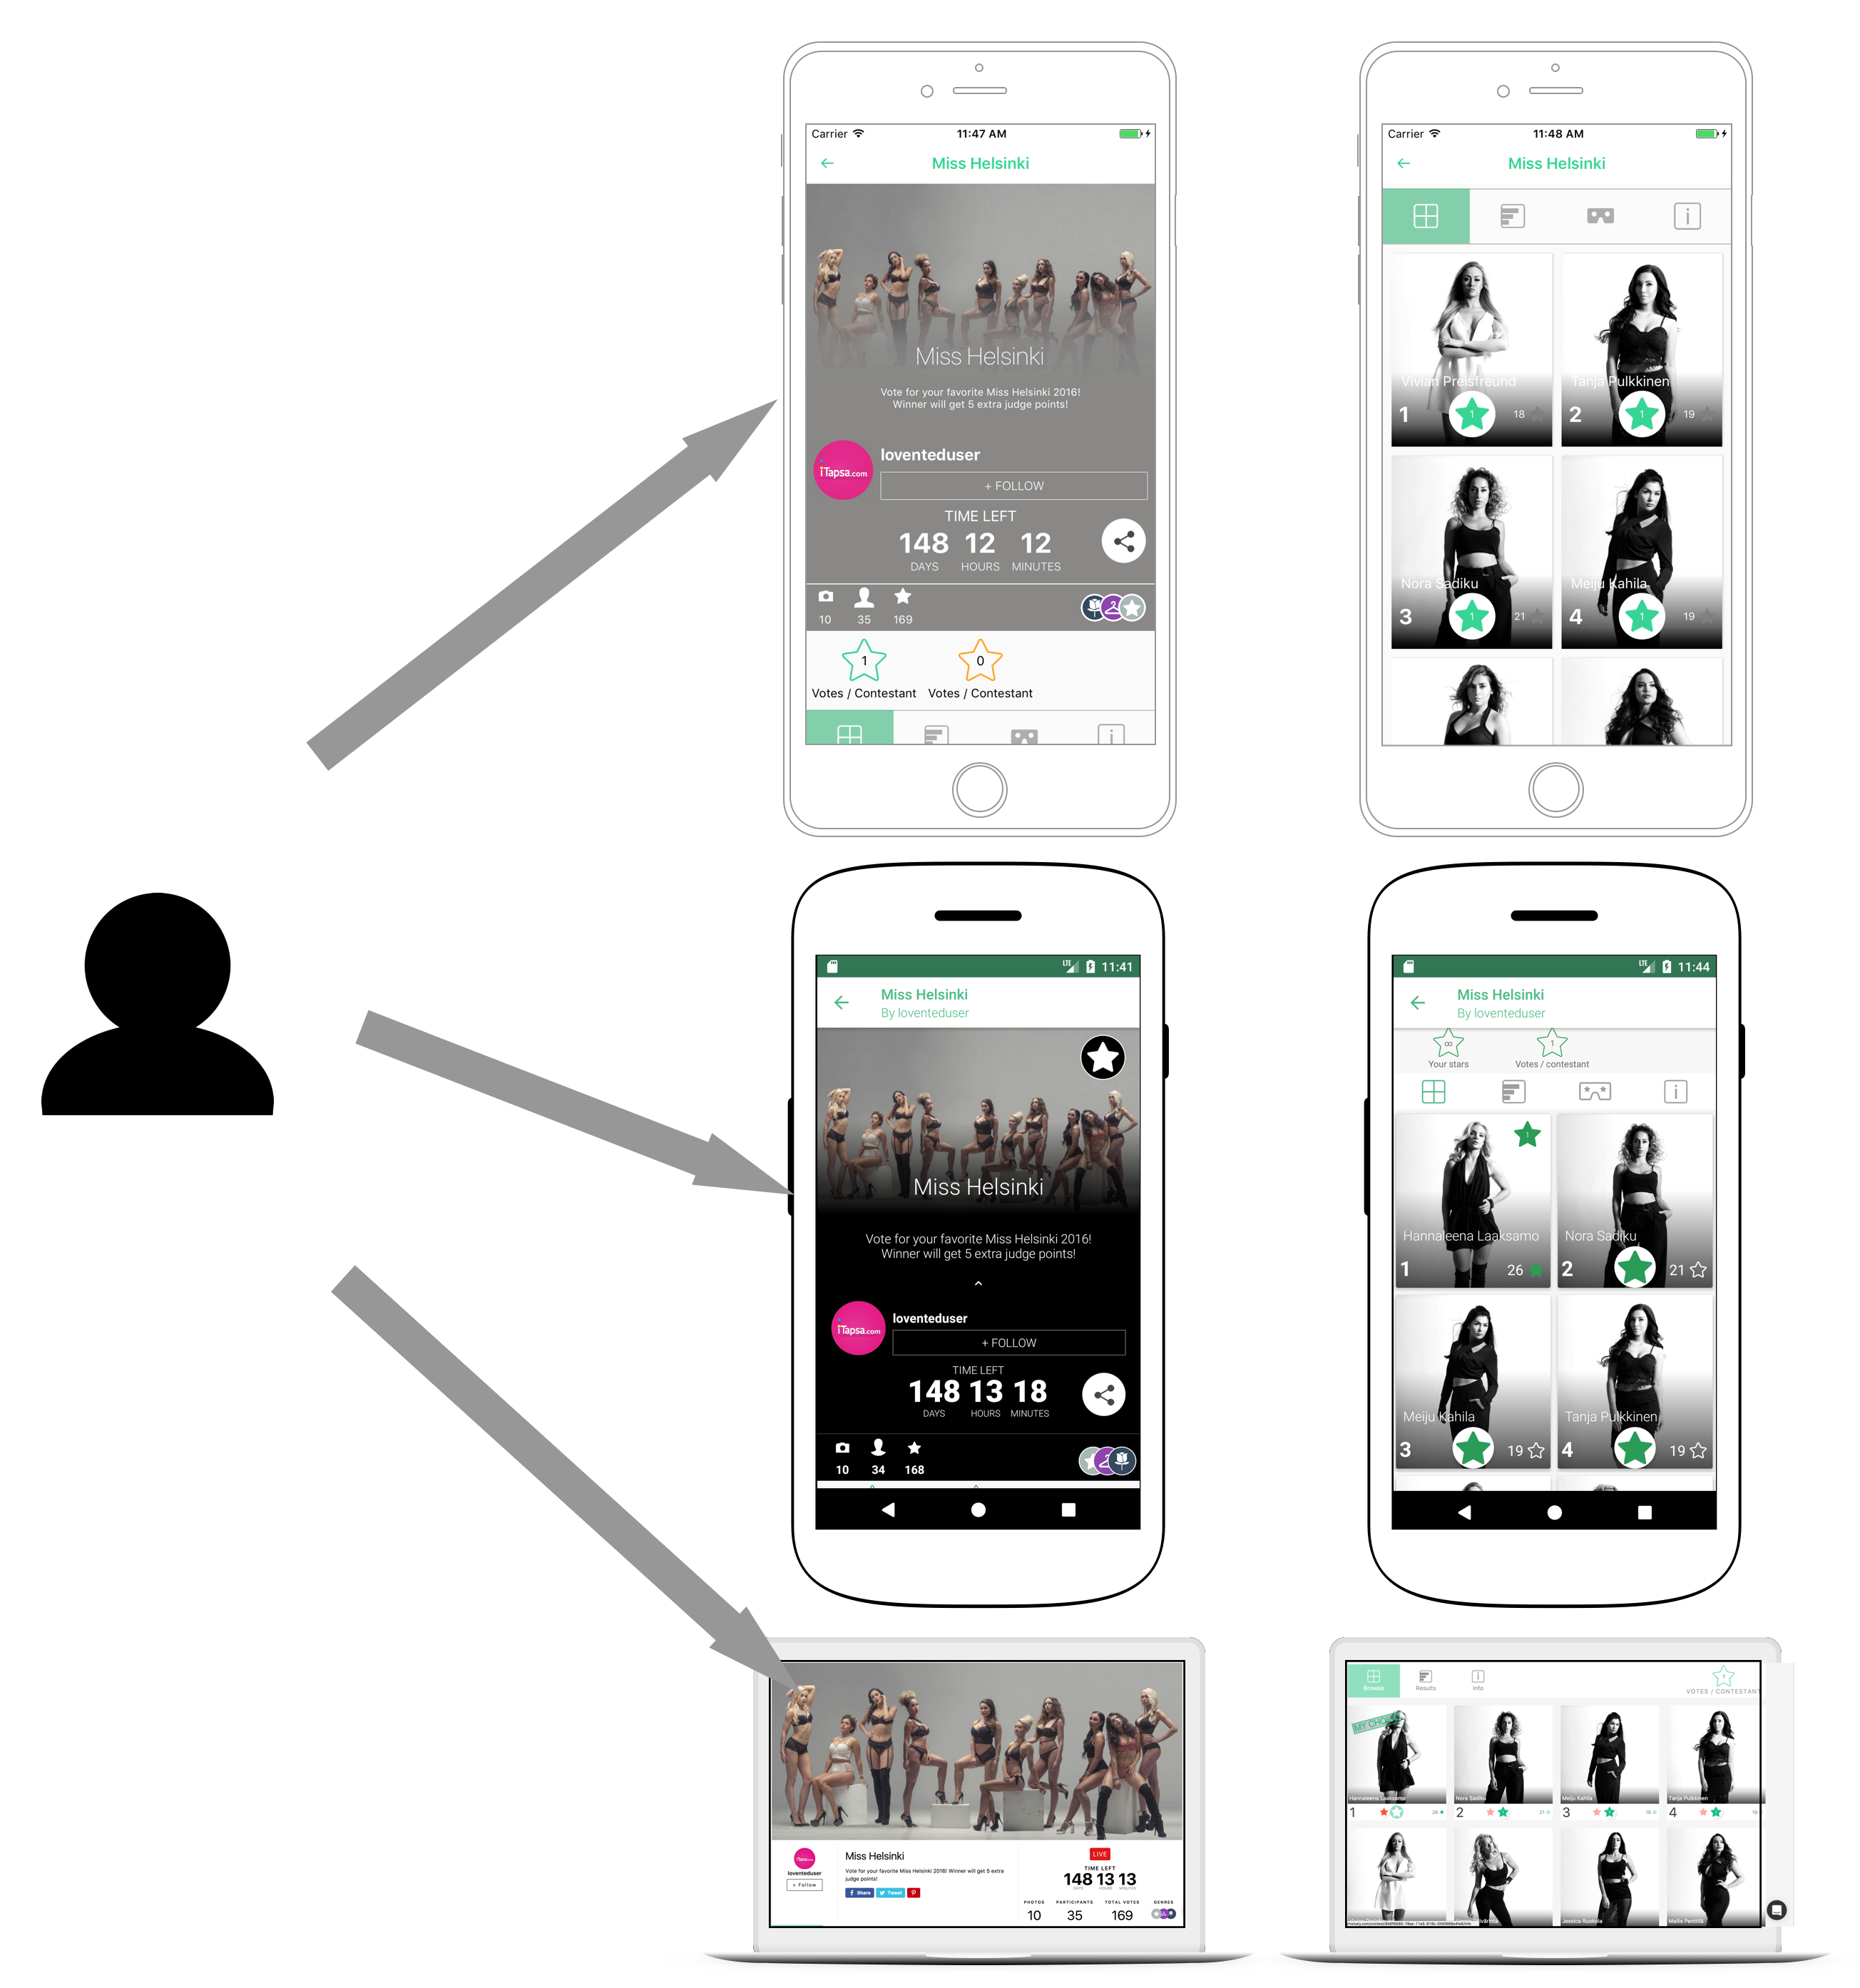
\includegraphics[width=0.6\textwidth]{images/choicely_platforms.png}
            \caption{Users can vote in contests through three interfaces: iOS devices, Android devices and web.}
            \label{choicely_platforms}
        \end{center}
    \end{figure}

    % what do users have to do to participate? 
    Majority of the contests require users to have a user profile in the Choicely platform. Choicely offers authentication through social media (Facebook and Google+) as a convenient option for users to sign up with one click. In this case, the social media platform provides information about the user's profile to Choicely, which allows the automatic population of the demographic data of the user. Optionally, user profiles in Choicely can be created through a regular sign-up process, where users pick a username as their identities. In such case, their demographic data is unknown by default and it is up to the users to complete their profiles. 
    % When users choose this kind of registration, their e-mail addresses are confirmed through a verification link sent to their inbox, so that their identity is confirmed. 

    % other contest-related data
    Contests also have some meta data which can facilitate data analysis. Each contest belongs to at least one but up to three of the following categories: animals, beauty, danger, design, entertainment, fashion, food, games, humor, sports, travel, other. The category labels are aligned by the contest's author upon creation. Contests also have starting and an ending time, between which users can vote or participate in them. While votes arrive into a contest, the vote count value tells the number of total votes received, while the number of unique voters tells how many individual users have voted in the contest. 

    \begin{figure}[h] 
        \begin{center}
            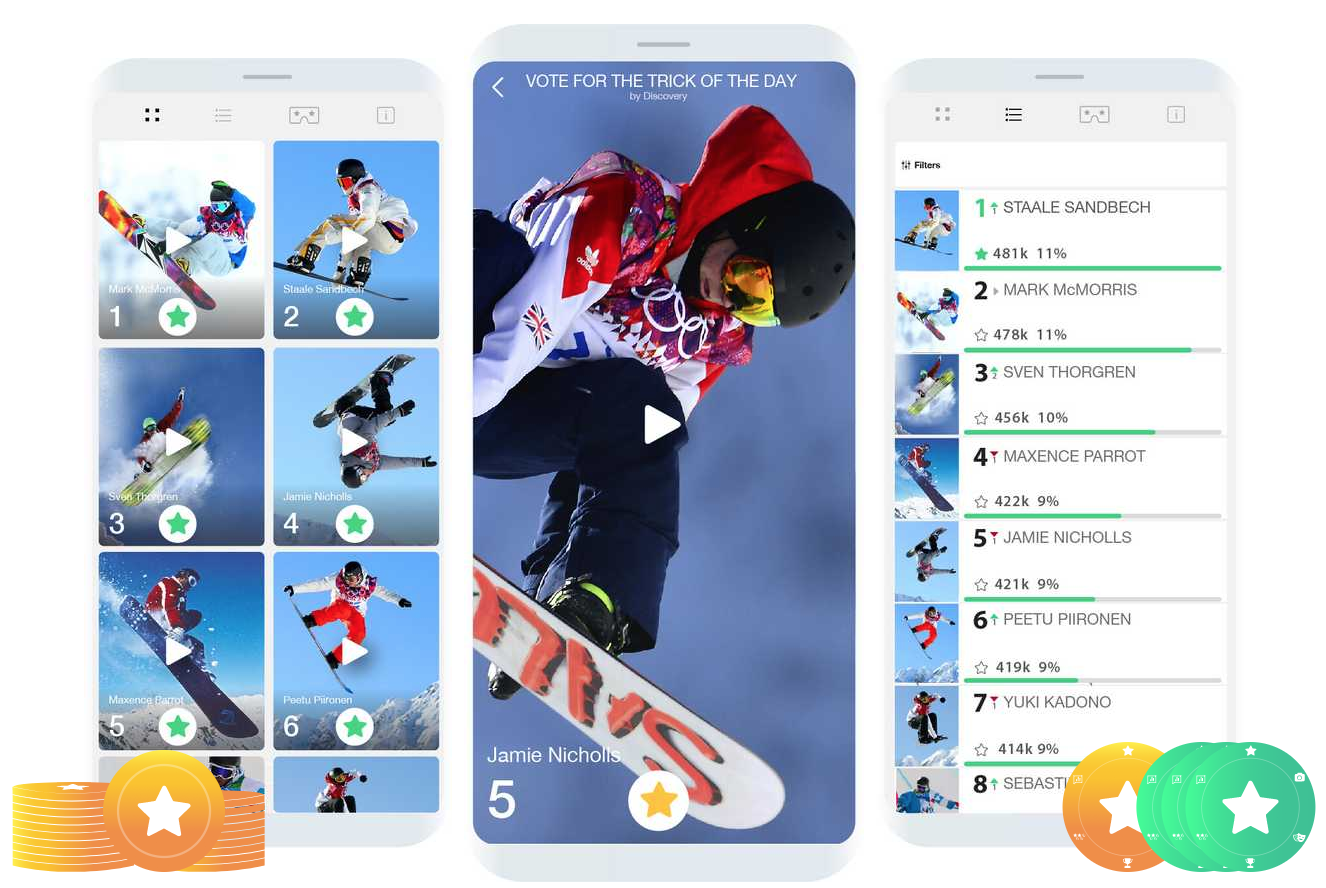
\includegraphics[width=0.6\textwidth]{images/vote_trick_of_the_day.png}
            % 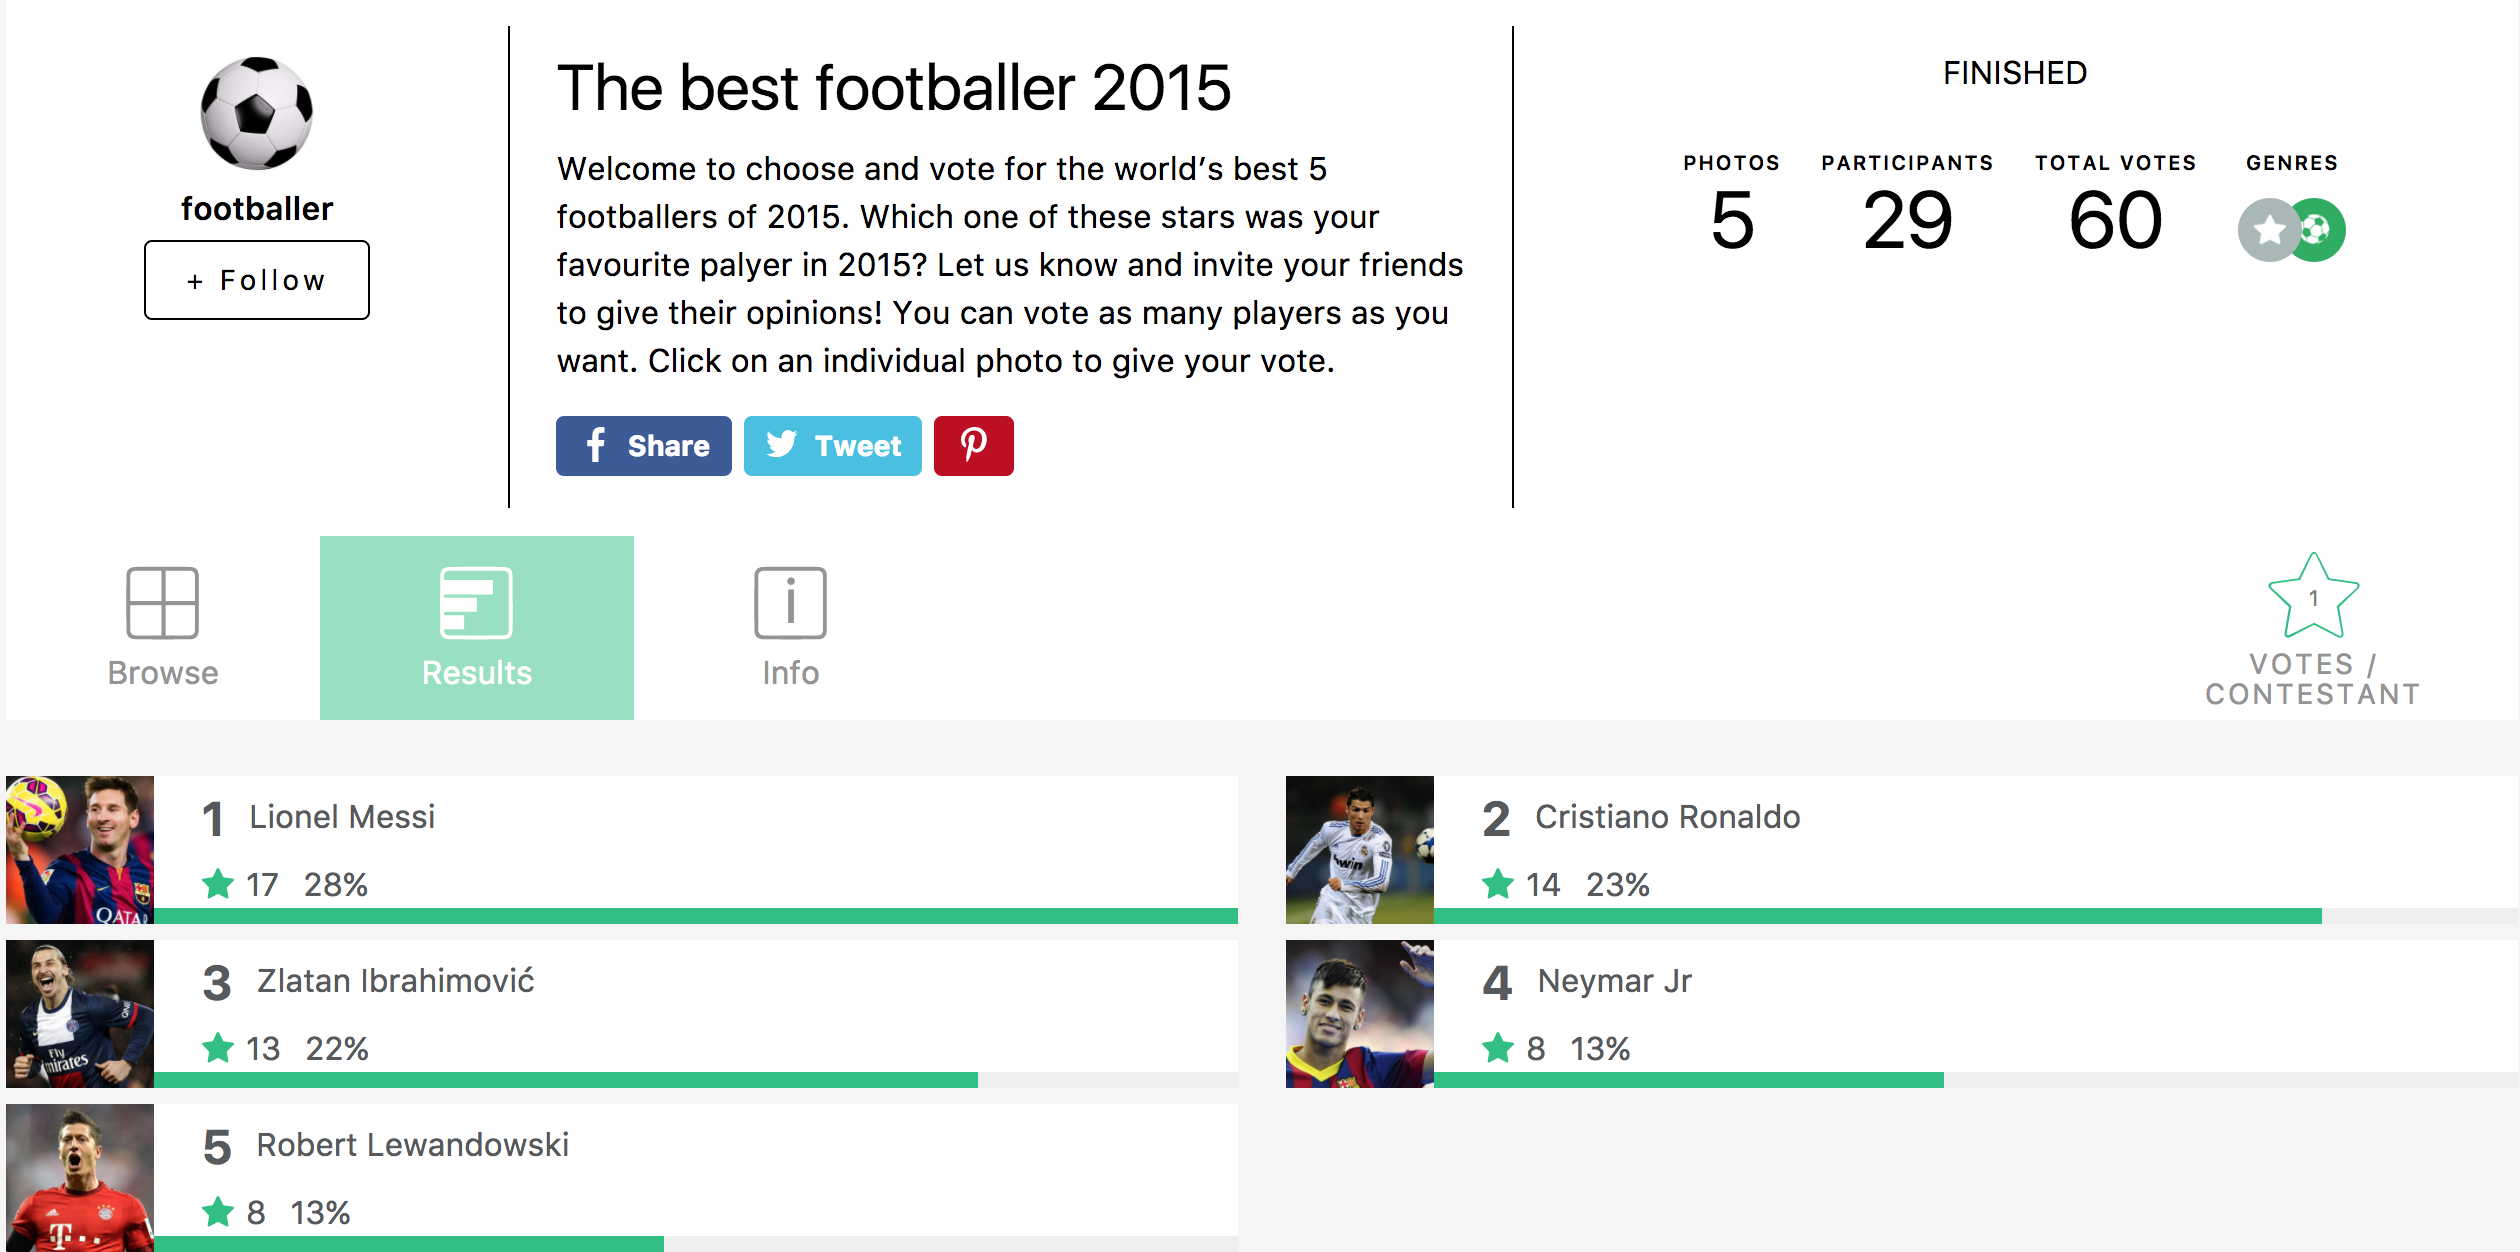
\includegraphics[width=0.6\textwidth]{images/best_footballer_2015_results.png}
            \caption{The visual appearance of a contest in Choicely.}
            \label{vote_trick_of_the_day}
        \end{center}
    \end{figure}

    % other contest participant-related data
    One important fact to highlight is, that the contestants have no meta data other than in which contest they are contending. Information about contestants is limited to the contest they contend in, their names, short descriptions, image and video. One of the limitations of the platform is to facilitate information about the contest participants and their traits. 
    
    % state some challenges
    There is currently no way of knowing if there is a tendency in what kind of participants tend to be more engaging to the audience. Secondly, there is yet no possibility to know if there would be a similarity or difference in target groups behavior in terms of what kind of content they spend votes on. The goal of this thesis work is to address these challenges by developing a data analysis framework for the company.

\subsection{Thesis structure}
    % how is the thesis structured? 
    This chapter presents the structure of this thesis work. First an overview on the theoretical background and on the related work in the field of audience engagement and user data analysis is presented. % TODO